% !TEX program = xelatex
\documentclass[11pt]{ctexart}
\usepackage[a4paper,left=2.0cm,right=2.0cm,top=2.0cm,bottom=2.2cm]{geometry}
\usepackage{amsmath,amssymb}
\usepackage{xcolor}
\usepackage{array}
\usepackage{enumitem}
\usepackage{tikz}
\usepackage{needspace}
\usetikzlibrary{arrows.meta,patterns,calc}

\setlist{nosep,leftmargin=1.7em}
\linespread{1.24}
\setlength{\parskip}{3pt}
\setlength{\parindent}{0pt}
\setlength{\tabcolsep}{5pt}
\renewcommand{\arraystretch}{1.22}

\definecolor{deepblue}{RGB}{12,82,160}
\definecolor{deepnavy}{RGB}{18,60,104}
\definecolor{band}{RGB}{242,246,251}
\definecolor{band2}{RGB}{250,247,238}
\definecolor{rulegray}{RGB}{200,212,228}
\definecolor{ansgreen}{RGB}{22,110,70}

\newcommand{\hdr}[1]{%
  \par\vspace{9pt}%
  \noindent{\color{deepblue}\large\bfseries #1}\par\vspace{2pt}%
  \noindent{\color{deepblue}\rule{\linewidth}{1.1pt}}\par\vspace{5pt}}

\newcommand{\boxednote}[1]{%
  \par\medskip\noindent
  \fcolorbox{rulegray}{band}{\parbox{\dimexpr\linewidth-2\fboxsep-2\fboxrule}{\vspace{2pt}#1\vspace{2pt}}}%
  \par\medskip}

\newcommand{\warnnote}[1]{%
  \par\medskip\noindent
  \fcolorbox{rulegray}{band2}{\parbox{\dimexpr\linewidth-2\fboxsep-2\fboxrule}{\vspace{2pt}#1\vspace{2pt}}}%
  \par\medskip}

\newcommand{\score}[2]{\par\vspace{3pt}\noindent{\color{deepblue}\bfseries 题 #1}\ {\small\color{deepnavy}｜#2}\par\vspace{2pt}}
\newcommand{\cnline}[1]{\par\noindent{\small\color{gray}题意：#1}\par\vspace{2pt}}
\newcommand{\solhdr}[1]{\par\vspace{3pt}\noindent{\color{ansgreen}\bfseries #1}\par\vspace{1pt}}
\newcommand{\ans}[1]{\par\medskip\noindent{\color{ansgreen}\bfseries 答案：}#1\par\medskip}
\newcommand{\vect}[1]{\boldsymbol{#1}}

\tikzset{
  dim/.style={<->,>=stealth,thin},
  vec/.style={->,>=stealth,thick,deepblue},
  obj/.style={thick},
  dashline/.style={dashed,thin,gray}
}

\begin{document}

\begin{center}
{\LARGE\bfseries 工程力学竞赛（亚洲赛区）选拔}\\[4pt]
{\LARGE\bfseries 模拟 A 卷：八道典型题}\\[8pt]
{\small 结构对齐个人赛：静力学 2 题 · 运动学 2 题 · 动力学 4 题；全英文题干，中文详解}\\[3pt]
{\small 建议限时 100 分钟完成第一部分，对答案后再看详解}\\[3pt]
{\small 整理日期 2026-10-19\quad｜\quad 全部答案已用 SymPy 验算}
\end{center}

\warnnote{\textbf{关于来源，说清楚}：以下 8 道题不是国际大学生工程力学竞赛的往届真题（真题卷未公开流传），而是按该赛事个人赛的\textbf{科目结构、题量与难度比例}编写的模拟题，考点覆盖标准理论力学的三块核心题库。用它练“在英文题干下认出该用哪个定理”这件事，比刷某一年的原卷更实用。}

%=====================================================================
\hdr{一、试卷结构与配时}

\begin{center}
\small
\begin{tabular}{|c|c|>{\raggedright\arraybackslash}p{5.6cm}|c|c|}
\hline
\textbf{题号} & \textbf{板块} & \textbf{考查点} & \textbf{难度} & \textbf{建议用时} \\ \hline
S1 & 静力学 & 摩擦平衡、极限状态 & 中 & 10 min \\ \hline
S2 & 静力学 & 桁架内力（节点法） & 中 & 12 min \\ \hline
K1 & 运动学 & 点的复合运动、科氏加速度、曲率半径 & 高 & 15 min \\ \hline
K2 & 运动学 & 刚体平面运动、瞬心、加速度分析 & 高 & 15 min \\ \hline
D1 & 动力学 & 定轴转动 + 平动的耦合 & 中 & 10 min \\ \hline
D2 & 动力学 & 拉格朗日方程、有效势、稳定性 & 高 & 15 min \\ \hline
D3 & 动力学 & 碰撞、冲量、能量损失 & 中 & 8 min \\ \hline
D4 & 动力学 & 有心力场、有效势、转向点 & 高 & 15 min \\ \hline
\end{tabular}
\end{center}

%=====================================================================
\newpage
\hdr{二、试题（English）}

\Needspace{9cm}
\score{S1}{静力学 · 摩擦平衡 · 12 marks}
\textit{A uniform ladder of length $L$ and weight $W$ rests with its upper end $B$ against a smooth vertical wall and its lower end $A$ on rough horizontal ground, the coefficient of static friction being $\mu$. The ladder makes an angle $\theta$ with the ground. Determine the smallest value of $\mu$ for which the ladder can remain in equilibrium, and discuss the limiting cases $\theta\to 90^\circ$ and $\theta\to 0$.}
\cnline{均质梯子斜靠光滑墙、地面有摩擦，求维持平衡所需的最小摩擦系数。}

\begin{center}
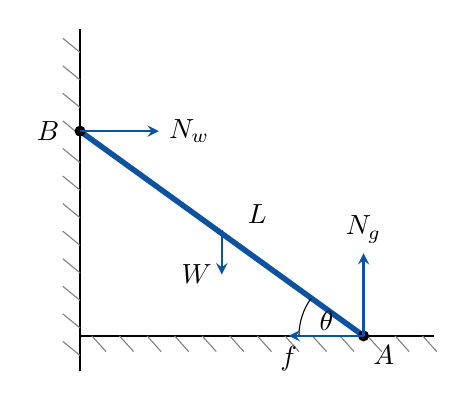
\begin{tikzpicture}[scale=1.0]
  % 墙（x=0）与地面（y=0）
  \draw[thick] (0,-0.45) -- (0,3.9);
  \foreach \y in {-0.25,0.1,...,3.8} \draw[thin,gray] (0,\y) -- (-0.22,\y+0.18);
  \draw[thick] (0,0) -- (4.5,0);
  \foreach \x in {0.15,0.5,...,4.4} \draw[thin,gray] (\x,0) -- (\x+0.18,-0.2);
  % 梯子
  \coordinate (A) at (3.6,0);
  \coordinate (B) at (0,2.6);
  \draw[line width=2pt,deepblue] (A) -- (B);
  \fill (A) circle (2pt); \fill (B) circle (2pt);
  \node[below right] at (A) {$A$};
  \node[left] at (-0.14,2.6) {$B$};
  % 角 theta
  \draw (2.78,0) arc (180:144.2:0.82);
  \node at (3.13,0.19) {$\theta$};
  % 受力
  \draw[vec] (1.8,1.34) -- (1.8,0.78) node[left,black,pos=1.0] {$W$};
  \draw[vec] (0,2.6) -- (1.0,2.6) node[right,black] {$N_w$};
  \draw[vec] (A) -- ++(0,1.05) node[above,black] {$N_g$};
  \draw[vec] (A) -- ++(-0.95,0) node[below,black] {$f$};
  \node[fill=white,inner sep=1pt] at (2.25,1.55) {$L$};
\end{tikzpicture}
\end{center}

\Needspace{9cm}
\score{S2}{静力学 · 桁架内力 · 13 marks}
\textit{A plane pin-jointed truss consists of three members $AB$, $BC$ and $CA$, with joints at $A(0,0)$, $B(4,0)$ and $C(2,3)$ in metres. Joint $A$ is a pin support and joint $B$ rests on a smooth horizontal roller. A vertical load $P$ acting downwards is applied at $C$. Neglecting the weights of the members, determine the axial force in each member and state whether it is tensile or compressive.}
\cnline{三点桁架，顶点集中载荷，求三根杆的内力与拉压性质（节点法）。}

\begin{center}
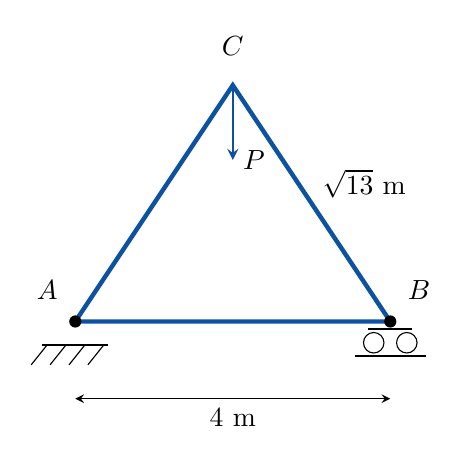
\begin{tikzpicture}[scale=1.0]
  \coordinate (A) at (0,0); \coordinate (B) at (4,0); \coordinate (C) at (2,3);
  \draw[line width=1.6pt,deepblue] (A) -- (B) -- (C) -- cycle;
  % A 处固定铰支座
  \fill (A) circle (2.2pt);
  \draw[thick] (-0.42,-0.3) -- (0.42,-0.3);
  \foreach \x in {-0.36,-0.12,0.12,0.36} \draw[thin] (\x,-0.3) -- (\x-0.2,-0.55);
  \node[above left] at (-0.1,0.15) {$A$};
  % B 处滚子支座
  \fill (B) circle (2.2pt);
  \draw[thick] (3.72,-0.1) -- (4.28,-0.1);
  \draw (3.79,-0.27) circle (0.13); \draw (4.21,-0.27) circle (0.13);
  \draw[thick] (3.55,-0.44) -- (4.45,-0.44);
  \node[above right] at (4.1,0.15) {$B$};
  % 载荷
  \draw[vec] (C) -- (2,2.05) node[right,black] {$P$};
  \node[above] at (2,3.25) {$C$};
  % 尺寸
  \draw[dim] (0,-0.98) -- (4,-0.98) node[midway,below] {$4\ \mathrm{m}$};
  \node[right,fill=white,inner sep=1pt] at (3.1,1.75) {$\sqrt{13}\ \mathrm{m}$};
\end{tikzpicture}
\end{center}

\Needspace{5cm}
\score{K1}{运动学 · 复合运动 · 15 marks}
\textit{A straight tube rotates in a horizontal plane about a vertical axis through its end $O$ with constant angular velocity $\omega$. A small particle slides along the tube away from $O$ with constant speed $u$ relative to the tube. At the instant when the particle is at a distance $r$ from $O$, determine (a) the magnitude of its absolute velocity, (b) the magnitude of its absolute acceleration, and (c) the radius of curvature of its path.}
\cnline{旋转管中匀速外滑的质点：绝对速度、绝对加速度（含科氏项）、轨迹曲率半径。}

\Needspace{9cm}
\score{K2}{运动学 · 刚体平面运动 · 15 marks}
\textit{A uniform rod $AB$ of length $L$ moves in a vertical plane with its end $A$ on a smooth horizontal guide (the $x$-axis) and its end $B$ on a smooth vertical guide (the $y$-axis). At the instant when the rod makes an angle $\theta$ with the horizontal, end $A$ is moving towards the origin with constant speed $v_A$. Determine (a) the angular velocity of the rod, (b) the velocity of end $B$, and (c) the acceleration of end $B$.}
\cnline{墙角里滑动的杆（A 在 x 轴、B 在 y 轴），A 匀速，求角速度、B 的速度与加速度。}

\begin{center}
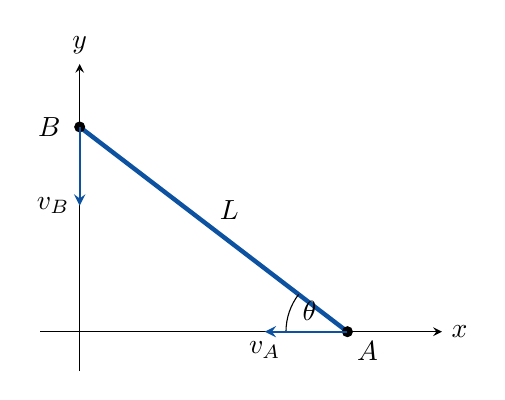
\begin{tikzpicture}[scale=1.0]
  \draw[->,>=stealth] (-0.5,0) -- (4.6,0) node[right] {$x$};
  \draw[->,>=stealth] (0,-0.5) -- (0,3.4) node[above] {$y$};
  \coordinate (A) at (3.4,0);
  \coordinate (B) at (0,2.6);
  \draw[line width=1.6pt,deepblue] (A) -- (B);
  \fill (A) circle (2pt); \fill (B) circle (2pt);
  \node[below right] at (A) {$A$};
  \node[left] at (-0.12,2.6) {$B$};
  % 角
  \draw (2.62,0) arc (180:142.6:0.78);
  \node at (2.92,0.26) {$\theta$};
  % 速度
  \draw[vec] (A) -- (2.35,0) node[below,black] {$v_A$};
  \draw[vec] (B) -- (0,1.6) node[left,black] {$v_B$};
  \node[fill=white,inner sep=1pt] at (1.9,1.55) {$L$};
\end{tikzpicture}
\end{center}

\Needspace{9cm}
\score{D1}{动力学 · 定轴转动 + 平动 · 10 marks}
\textit{A uniform solid cylinder of mass $M$ and radius $R$ can rotate without friction about its fixed horizontal axis. A light inextensible string, wound round the cylinder, carries a particle of mass $m$ at its free end. The system is released from rest. Determine (a) the acceleration of the particle, (b) the tension in the string, and (c) the resultant force exerted by the axle on the cylinder.}
\cnline{细绳绕在圆柱上吊一个质量，求下落加速度、绳张力、轴承反力。}

\begin{center}
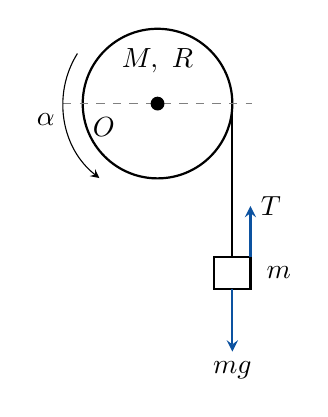
\begin{tikzpicture}[scale=1.0]
  \draw[thick] (0,0) circle (0.95);
  \draw[dashline] (-1.2,0) -- (1.2,0);
  \fill (0,0) circle (2.5pt);
  \node[below left] at (-0.42,-0.06) {$O$};
  \node at (0,0.55) {$M,\ R$};
  % 细绳与吊块
  \draw[thick] (0.95,0) -- (0.95,-1.95);
  \draw[thick] (0.72,-1.95) rectangle (1.18,-2.35);
  \node[right] at (1.26,-2.15) {$m$};
  \draw[vec] (0.95,-2.35) -- (0.95,-3.15) node[below,black] {$mg$};
  \draw[vec] (1.18,-1.95) -- (1.18,-1.3) node[right,black] {$T$};
  % 角加速度（绕轴的弧形箭头）
  \draw[->,>=stealth] (148:1.2) arc (148:232:1.2) node[pos=0.5,left,black] {$\alpha$};
\end{tikzpicture}
\end{center}

\Needspace{9cm}
\score{D2}{动力学 · 拉格朗日 + 有效势 + 稳定性 · 15 marks}
\textit{A bead slides without friction on a smooth circular wire hoop of radius $R$. The hoop is made to rotate about its vertical diameter with constant angular velocity $\omega$. Let $\theta$ denote the angle between the radius drawn to the bead and the downward vertical. (a) Find all equilibrium positions of the bead relative to the hoop; (b) determine the stability of each position; (c) describe how the (stable) equilibrium position varies as $\omega$ increases from zero.}
\cnline{旋转竖直圆环上的珠子：找相对平衡位置、判稳定性、看随 $\omega$ 变化的分岔。}

\begin{center}
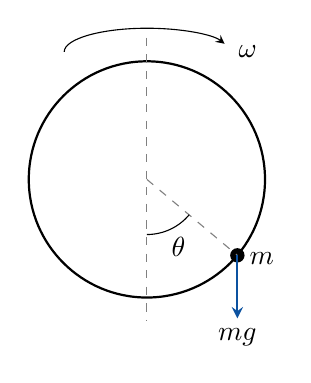
\begin{tikzpicture}[scale=1.0]
  \draw[thick] (0,0) circle (1.5);
  \draw[dashline] (0,1.8) -- (0,-1.8);
  % 绕竖直轴转动的示意箭头
  \draw[->,>=stealth] (-1.05,1.62) arc (180:20:1.05 and 0.3);
  \node at (1.28,1.62) {$\omega$};
  % 珠子
  \coordinate (P) at (-40:1.5);
  \fill (P) circle (2.6pt);
  \draw[dashline] (0,0) -- (P);
  \draw (0,-0.7) arc (270:320:0.7);
  \node at (0.40,-0.86) {$\theta$};
  \node[right] at (1.18,-1.0) {$m$};
  \draw[vec] (P) -- ++(0,-0.8) node[below,black] {$mg$};
\end{tikzpicture}
\end{center}

\Needspace{9cm}
\score{D3}{动力学 · 碰撞与冲量 · 10 marks}
\textit{A particle of mass $m$ strikes a smooth vertical wall with speed $v$, the direction of its velocity making an angle of $45^\circ$ with the normal to the wall. The coefficient of restitution between the particle and the wall is $e$. Determine (a) the impulse exerted by the wall on the particle, and (b) the fraction of the initial kinetic energy that is lost during the impact.}
\cnline{45° 斜碰光滑墙，恢复系数 e：求冲量大小与动能损失的相对比例。}

\begin{center}
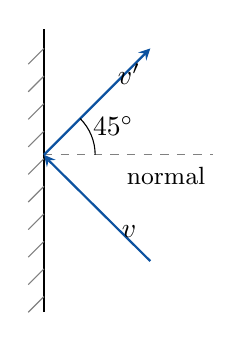
\begin{tikzpicture}[scale=1.0]
  % 墙（x=0，材料在左侧）
  \draw[thick] (0,-0.3) -- (0,3.3);
  \foreach \y in {-0.1,0.25,...,3.2} \draw[thin,gray] (0,\y) -- (-0.2,\y-0.2);
  % 法线
  \draw[dashline] (0,1.7) -- (2.15,1.7);
  \node[below] at (1.55,1.66) {\small normal};
  % 入射（与法线成 45 度）与反射
  \draw[vec] (1.35,0.35) -- (0,1.7);
  \draw[vec] (0,1.7) -- (1.35,3.05);
  \node[black] at (1.08,0.72) {$v$};
  \node[black] at (1.08,2.72) {$v'$};
  \draw (0.65,1.7) arc (0:45:0.65);
  \node at (0.88,2.06) {$45^\circ$};
\end{tikzpicture}
\end{center}

\Needspace{5cm}
\score{D4}{动力学 · 有心力场 · 10 marks}
\textit{A particle of mass $m$ moves in the attractive central field $U(r)=-k/r$ ($k>0$) with angular momentum $L$ and negative total energy $E<0$. (a) Show that the radial motion is bounded and find the two apsidal (turning) distances $r_{\min}$, $r_{\max}$. (b) Find the condition for the orbit to be a circle, and the radius of that circle in terms of $L$, $m$, $k$. (c) Find the period of the circular orbit.}
\cnline{万有引力型有心力场：证明径向有界、求两个转向点、圆轨道条件与半径、圆轨道周期。}

%=====================================================================
\hdr{三、答案速览（先自己做完再核对）}

\begin{center}
\small
\begin{tabular}{|c|>{\raggedright\arraybackslash}p{4.6cm}|>{\raggedright\arraybackslash}p{8.6cm}|}
\hline
\textbf{题号} & \textbf{所求量} & \textbf{结果} \\ \hline
S1 & 最小摩擦系数 & $\mu_{\min}=\dfrac{1}{2\tan\theta}=\dfrac{\cot\theta}{2}$ \\ \hline
S2 & 三杆内力 & $N_{AC}=N_{BC}=-\dfrac{\sqrt{13}}{6}P$（压），$N_{AB}=+\dfrac{P}{3}$（拉） \\ \hline
K1 & 速度、加速度、曲率半径 & $\lvert \vect{v}\rvert=\sqrt{u^2+\omega^2r^2}$，$\lvert \vect{a}\rvert=\omega\sqrt{\omega^2r^2+4u^2}$，$\rho=\dfrac{(u^2+\omega^2r^2)^{3/2}}{\omega\,(\omega^2r^2+2u^2)}$ \\ \hline
K2 & $\omega$, $v_B$, $a_B$ & $\omega=\dfrac{v_A}{L\sin\theta}$，$v_B=v_A\cot\theta$，$a_B=\dfrac{v_A^2}{L\sin^3\theta}$（指向原点） \\ \hline
D1 & $a$, $T$, 轴反力 & $a=\dfrac{2mg}{M+2m}$，$T=\dfrac{Mmg}{M+2m}$，$R_{\mathrm{axle}}=Mg\Big(1+\dfrac{m}{M+2m}\Big)$ \\ \hline
D2 & 平衡位置与稳定性 & $\theta=0$ 恒为平衡；$\omega^2R>g$ 时另有 $\theta^*=\arccos\dfrac{g}{\omega^2R}$ \\ \hline
D3 & 冲量、动能损失比 & $J=\dfrac{mv(1+e)}{\sqrt2}$，$\dfrac{\Delta K}{K_0}=\dfrac{1-e^2}{2}$ \\ \hline
D4 & 转向点、圆轨道、周期 & $r_{\min,\max}=\dfrac{k\mp\sqrt{k^2+2EL^2/m}}{2\lvert E\rvert}$，圆轨道 $E=-\dfrac{mk^2}{2L^2}$、$r_0=\dfrac{L^2}{mk}$、$T=\dfrac{2\pi L^3}{mk^2}$ \\ \hline
\end{tabular}
\end{center}

%=====================================================================
\hdr{四、详解}

\solhdr{S1\quad 摩擦平衡：一个方程解决“极限”}

受力共四个：重力 $W$（作用在中点，竖直向下）、墙的支持力 $N_w$（水平，指向外）、地面的支持力 $N_g$（竖直向上）、地面摩擦力 $f$（指向墙，阻止下滑）。

竖直、水平方向平衡：

\[
N_g=W,\qquad f=N_w
\]

对 $A$ 点取矩（这样 $N_g$、$f$ 都不产生力矩）：

\[
W\cdot\frac{L}{2}\cos\theta=N_w\cdot L\sin\theta
\quad\Longrightarrow\quad
N_w=\frac{W}{2\tan\theta}
\]

不打滑的临界条件是 $f\le\mu N_g$，即 $N_w\le\mu W$，代入上式：

\[
\boxed{\ \mu_{\min}=\frac{1}{2\tan\theta}=\frac{\cot\theta}{2}\ }
\]

\textbf{两个极限的物理含义}：$\theta\to 90^\circ$ 时 $\mu_{\min}\to 0$——梯子立直时重力线几乎落在支点正上方，不需要摩擦；$\theta\to 0$ 时 $\mu_{\min}\to\infty$——躺平的梯子靠墙也撑不住，必然滑倒。另外注意结果与 $L$、$W$ 都无关，只由几何角与摩擦决定，这是这类题的常见结论形式。

\solhdr{S2\quad 桁架：先整体求反力，再逐个节点封闭}

\textbf{第一步：整体平衡}。结构对称、载荷在对称轴上，所以两支座竖向反力相等、水平反力为零：

\[
R_{Ay}=R_{By}=\frac{P}{2},\qquad R_{Ax}=0
\]

\textbf{第二步：节点 $C$}（两根杆 + 外载）。设 $S_{AC}$、$S_{BC}$ 为杆的轴向力（\textbf{拉为正}），杆的方向分别为

\[
\vect{u}_{CA}=\frac{(-2,-3)}{\sqrt{13}},\qquad \vect{u}_{CB}=\frac{(2,-3)}{\sqrt{13}}
\]

节点 $C$ 的平衡：

\[
S_{AC}\vect{u}_{CA}+S_{BC}\vect{u}_{CB}+(0,-P)=\vect 0
\]

$x$ 方向给出 $S_{AC}=S_{BC}=S$，$y$ 方向给出

\[
-\frac{6S}{\sqrt{13}}=P\quad\Longrightarrow\quad S=-\frac{\sqrt{13}}{6}P
\]

负号表示\textbf{受压}，大小为 $\sqrt{13}P/6\approx0.601P$。

\textbf{第三步：节点 $A$}（两根杆 + 支座反力）。压杆 $AC$ 给节点的力指向 $C$，写成 $S_{AC}\vect u_{AC}$；沿 $x$ 方向投影时，$A$ 处没有水平支座反力，故

\[
S_{AB}+\frac{2}{\sqrt{13}}S_{AC}=0
\quad\Longrightarrow\quad
S_{AB}=-\frac{2}{\sqrt{13}}\cdot\left(-\frac{\sqrt{13}}{6}P\right)=\frac{P}{3}
\]

（$y$ 方向可以抽查：$\dfrac{P}{2}-\dfrac{3}{\sqrt{13}}\cdot\dfrac{\sqrt{13}}{6}P=\dfrac{P}{2}-\dfrac{P}{2}=0$，节点确实平衡。）

\ans{$N_{AC}=N_{BC}=-\dfrac{\sqrt{13}}{6}P$（受压），$N_{AB}=+\dfrac{P}{3}$（受拉）。}

\warnnote{\textbf{这一类题的通用节奏}：先整体（三个平衡方程解支座反力）→ 再挑“未知力不超过两个”的节点开始解 → 最后抽查另一个节点验证。若题意要求找“零杆”，看该节点是否只有两根不共线的杆且无外载。}

\solhdr{K1\quad 复合运动：三个速度、三个加速度，一项都别漏}

管在水平面内绕竖直轴转动，取固连于管的转动坐标系。质点在管中相对速度沿管向外，大小恒为 $u$；牵连速度由转动给出，方向垂直于管，大小 $\omega r$。两者垂直，所以

\[
\lvert\vect v\rvert=\sqrt{u^2+(\omega r)^2}
\]

加速度由三项组成：

\begin{itemize}
\item 相对加速度 $\vect a_r=\vect 0$（相对速度大小恒定、路径是直线）；
\item 牵连加速度 $\vect a_t=\omega^2 r$，指向转轴（向心）；
\item 科氏加速度 $\vect a_c=2\vect\omega\times\vect v_r$，大小 $2\omega u$，方向垂直于管（横向）。
\end{itemize}

向着转轴的分量与横向分量互相垂直，故

\[
\lvert\vect a\rvert=\sqrt{(\omega^2r)^2+(2\omega u)^2}=\omega\sqrt{\omega^2r^2+4u^2}
\]

曲率半径用 $\rho=v^3/\lvert v_\perp\rvert$ 的等价形式 $\rho=\lvert v\rvert^3/\lvert\vect v\times\vect a\rvert$。在（径向，横向）坐标下 $\vect v=(u,\omega r)$、$\vect a=(-\omega^2r,2\omega u)$，

\[
\lvert\vect v\times\vect a\rvert=\omega(2u^2+\omega^2r^2)
\quad\Longrightarrow\quad
\rho=\frac{(u^2+\omega^2r^2)^{3/2}}{\omega(2u^2+\omega^2r^2)}
\]

\textbf{易错}：漏掉科氏项（只写向心）是最常见的失分；另外 $2\vect\omega\times\vect v_r$ 的方向要按右手定则判断，本题里它指向运动前方（横向）。

\solhdr{K2\quad 墙角滑杆：一个约束方程，两次求导}

约束是杆长不变，故两端坐标满足

\[
x_A^2+y_B^2=L^2,\qquad x_A=L\cos\theta,\quad y_B=L\sin\theta
\]

\textbf{(a)} 对时间求导：$2x_A\dot x_A+2y_B\dot y_B=0$。由 $x_A=L\cos\theta$ 得 $\dot x_A=-L\sin\theta\,\dot\theta=-v_A$，于是

\[
\dot\theta=-\frac{v_A}{L\sin\theta}\quad\Longrightarrow\quad
\omega=\lvert\dot\theta\rvert=\frac{v_A}{L\sin\theta}
\]

\textbf{(b)} 代入速度关系：

\[
\dot y_B=-\frac{x_A}{y_B}\dot x_A=-v_A\cot\theta
\]

负号表示 $B$ 向下（朝原点）运动，速率 $v_A\cot\theta$。

\textbf{(c)} 再求导一次。由 $\dot x_A=-v_A$ 为常数得 $\ddot x_A=0$：

\[
\ddot x_A=-L\cos\theta\,\dot\theta^2-L\sin\theta\,\ddot\theta=0
\ \Longrightarrow\
\ddot\theta=-\cot\theta\,\dot\theta^2
\]

于是

\[
a_B=\ddot y_B=L(\cos\theta\,\ddot\theta-\sin\theta\,\dot\theta^2)
=-\frac{L\dot\theta^2}{\sin\theta}
=-\frac{v_A^2}{L\sin^3\theta}
\]

负号表示加速度朝原点（向下）。

\ans{$\omega=\dfrac{v_A}{L\sin\theta}$；$\lvert v_B\rvert=v_A\cot\theta$（向下）；$\lvert a_B\rvert=\dfrac{v_A^2}{L\sin^3\theta}$（向下）。}

\textbf{数值感受}：取 $L=1$ m、$v_A=2$ m/s、$\theta=30^\circ$，得 $\omega=4$ rad/s、$v_B\approx3.46$ m/s、$a_B=32$ m/s$^2$——注意 $A$ 是匀速的，但 $B$ 的加速度可以很大，因为 $\theta\to0$ 时 $\sin^3\theta$ 趋于零。

\solhdr{D1\quad 圆柱 + 吊块：两个方程，别忘转动惯量}

设吊块加速度 $a$（向下）、绳张力 $T$、圆柱角加速度 $\alpha$，圆柱转动惯量 $I=\frac12MR^2$。平动与转动方程：

\[
mg-T=ma,\qquad TR=I\alpha=\frac12MR^2\cdot\frac{a}{R}
\]

由第二式得 $T=\frac12Ma$，代入第一式：

\[
a=\frac{2mg}{M+2m},\qquad T=\frac{Mmg}{M+2m}
\]

轴反力：圆柱质心不动，竖直方向受自身重力 $Mg$、绳子向下的拉力 $T$、轴的支持力 $R_{\mathrm{axle}}$，故

\[
R_{\mathrm{axle}}=Mg+T=Mg\left(1+\frac{m}{M+2m}\right)=Mg\cdot\frac{M+3m}{M+2m}
\]

\textbf{数值检查}：$M=2$ kg、$m=1$ kg、$g=9.8$，得 $a=4.9$ m/s$^2$、$T=4.9$ N、$R_{\mathrm{axle}}=24.5$ N。可以顺手验算：$mg-T=9.8-4.9=4.9=ma$（成立）。

\solhdr{D2\quad 旋转圆环上的珠子：拉格朗日 → 有效势 → 二阶判据}

\textbf{第一步：写拉格朗日量}。珠子速度的平方由两个分量组成：沿环的 $R\dot\theta$，以及绕轴转动的 $R\sin\theta\cdot\omega$：

\[
T=\frac12mR^2\dot\theta^2+\frac12m\omega^2R^2\sin^2\theta
\]

取环心为零势能点，$U=-mgR\cos\theta$（$\theta$ 从最低点量起），于是

\[
L=\frac12mR^2\dot\theta^2+\frac12m\omega^2R^2\sin^2\theta+mgR\cos\theta
\]

\textbf{第二步：拉格朗日方程}（注意 $\partial L/\partial\dot\theta$ 只含 $\dot\theta$ 项）：

\[
mR^2\ddot\theta=m\omega^2R^2\sin\theta\cos\theta-mgR\sin\theta
\quad\Longrightarrow\quad
R\ddot\theta=\left(\omega^2R\cos\theta-g\right)\sin\theta
\]

\textbf{第三步：平衡 = 有效势的驻点}。在相对转动系里，离心惯性力可以并进势能：

\[
U_{\mathrm{eff}}(\theta)=-mgR\cos\theta-\frac12m\omega^2R^2\sin^2\theta,
\qquad
\frac{dU_{\mathrm{eff}}}{d\theta}=mR\left(g-\omega^2R\cos\theta\right)\sin\theta
\]

驻点给两个解：

\[
\sin\theta=0\ \Rightarrow\ \theta=0;
\qquad
\cos\theta=\frac{g}{\omega^2R}\ \Rightarrow\ \theta^*=\arccos\frac{g}{\omega^2R}\ (\text{仅当}\ \omega^2R>g)
\]

\textbf{第四步：稳定性判据}（$U_{\mathrm{eff}}''>0$ 为稳定）：

\[
U_{\mathrm{eff}}''=mR\left(g\cos\theta-2\omega^2R\cos^2\theta+\omega^2R\right)
\]

在 $\theta=0$：$U_{\mathrm{eff}}''\big|_0=mR(g-\omega^2R)$，所以

\[
\omega^2<\frac{g}{R}\ \text{时稳定},\qquad \omega^2>\frac{g}{R}\ \text{时不稳定}
\]

在 $\theta^*$（存在时）：代入 $\cos\theta^*=g/(\omega^2R)$ 得

\[
U_{\mathrm{eff}}''\big|_{\theta^*}=\frac{m\left(\omega^4R^2-g^2\right)}{\omega^2}>0\quad(\text{因为}\ \omega^2R>g)
\]

故 $\theta^*$ 总是稳定的。\textbf{临界角速度} $\omega_c=\sqrt{g/R}$ 处发生分岔（pitchfork bifurcation）：$\omega<\omega_c$ 时珠子稳在最低点；$\omega>\omega_c$ 时最低点失稳，珠子稳定在 $\theta^*$ 处，且 $\omega$ 越大 $\theta^*$ 越接近 $90^\circ$。

\ans{$\theta=0$ 恒为平衡位置，$\omega^2<g/R$ 稳定、$\omega^2>g/R$ 不稳定；若 $\omega^2R>g$ 还另有 $\theta^*=\arccos\dfrac{g}{\omega^2R}$，该位置稳定。}

\solhdr{D3\quad 45° 斜碰：法向用冲量，切向保持不变}

取法向（水平）与切向（沿墙）分解，初速度分量 $v_n=v\cos45^\circ=v/\sqrt2$、$v_t=v\sin45^\circ=v/\sqrt2$。

\textbf{(a)} 墙光滑，切向无冲量，$v_t$ 不变；法向按恢复系数反转，$v_n'=-ev_n$。法向冲量：

\[
J=m v_n-m(-ev_n)=mv_n(1+e)=\frac{mv(1+e)}{\sqrt2}
\]

\textbf{(b)} 碰后速度的平方 $v'^2=e^2v_n^2+v_t^2=\dfrac{v^2}{2}(1+e^2)$，故

\[
\frac{\Delta K}{K_0}=\frac{\frac12mv^2-\frac12mv'^2}{\frac12mv^2}
=1-\frac{1+e^2}{2}=\frac{1-e^2}{2}
\]

\textbf{数值}：$m=1$ kg、$v=10$ m/s、$e=0.5$ 时 $J\approx10.6$ N·s，动能损失 $37.5\%$。

\solhdr{D4\quad $-k/r$ 场的转向点与圆轨道：一个二次方程解决全部}

\textbf{(a)} 能量与角动量守恒，径向速度满足

\[
E=\frac12m\dot r^2+\frac{L^2}{2mr^2}-\frac{k}{r}
\quad\Longrightarrow\quad
E=-\frac{k}{r}+\frac{L^2}{2mr^2}\ \ (\text{转向点}\ \dot r=0)
\]

乘 $r^2$ 得 $E r^2+k r-\dfrac{L^2}{2m}=0$，两个正根即转向点：

\[
r_{\min,\max}=\frac{k\mp\sqrt{k^2+2EL^2/m}}{2\lvert E\rvert}
\]

有解（实数）的条件是判别式非负：

\[
k^2+\frac{2EL^2}{m}\ge0
\quad\Longleftrightarrow\quad
E\ge-\frac{mk^2}{2L^2}
\]

因为 $E<0$，这就是“$E$ 不能太低”的上界形式：当 $E$ 低于该值时径向方程无解，粒子落入中心。两个转向点都存在说明径向有两个限制，运动有界。

\textbf{(b)} 圆轨道的条件是两个转向点重合，即判别式为零：

\[
k^2+\frac{2EL^2}{m}=0
\quad\Longrightarrow\quad
E_{\mathrm{circ}}=-\frac{mk^2}{2L^2},
\qquad
r_0=\frac{k}{2\lvert E_{\mathrm{circ}}\rvert}=\frac{L^2}{mk}
\]

\textbf{(c)} 圆轨道上向心力由场力提供：$mv^2/r_0=k/r_0^2$，得 $v=\sqrt{k/(mr_0)}$，于是

\[
T=\frac{2\pi r_0}{v}=2\pi r_0\sqrt{\frac{mr_0}{k}}
=2\pi\cdot\frac{L^2}{mk}\cdot\frac{L}{k}
=\frac{2\pi L^3}{mk^2}
\]

\textbf{顺带一句}：$T\propto L^3$ 正是开普勒第三定律的“平方反比场版本”——周期只由角动量决定，与偏心率无关。这类题在竞赛里常以“证明/推导”形式出现，写出有效势再令分母为零是通法。

%=====================================================================
\hdr{五、自评表与错因定位}

做完后按下面这张表打分，把失分归类——比重做一遍题有用得多。

\begin{center}
\small
\begin{tabular}{|c|c|c|>{\raggedright\arraybackslash}p{3.2cm}|>{\raggedright\arraybackslash}p{3.6cm}|}
\hline
\textbf{题号} & \textbf{满分} & \textbf{得分} & \textbf{若失分，属于哪类} & \textbf{补救动作} \\ \hline
S1 & 12 & & 受力图画不全 / 力矩轴选错 & 重画受力图，只写 3 个方程 \\ \hline
S2 & 13 & & 整体反力漏水平分量 / 节点符号 & 用“拉正压负”统一约定再重算 \\ \hline
K1 & 15 & & 漏科氏项 / 方向判错 & 默写 $\vect a=\vect a_r+\vect a_t+\vect a_c$ \\ \hline
K2 & 15 & & 忘了“$v_A$ 恒定 $\Rightarrow$ $\ddot x_A=0$” & 二次求导时把该条件写出来 \\ \hline
D1 & 10 & & 转动惯量写错 / 漏轴反力 & 记住 $I=\frac12MR^2$ 与 $R=Mg+T$ \\ \hline
D2 & 15 & & 拉格朗日量少离心项 / 判据用错 & 用 $U_{\mathrm{eff}}''>0$ 重判一次 \\ \hline
D3 & 10 & & 切向也乘 $e$ / 能量算错 & 记住“光滑面切向不变” \\ \hline
D4 & 10 & & 二次方程根写错 / 忘了判别式条件 & 写成 $Er^2+kr-\frac{L^2}{2m}=0$ 再解 \\ \hline
\end{tabular}
\end{center}

\boxednote{\textbf{英文题干的高频句型}（读题时先抓这几个“动词+条件”）：\\
\textbf{Determine / Find / Obtain} —— 要你算出来，必须给表达式或数值；\\
\textbf{Neglecting friction / smooth surface} —— 该方向无摩擦，不要多写一个 $f$；\\
\textbf{The coefficient of restitution between \dots\ is $e$} —— 碰撞题唯一需要的额外参数；\\
\textbf{released from rest / moves with constant speed} —— 初条件或运动约束，往往决定某个导数为零；\\
\textbf{Show that \dots\ and hence obtain \dots} —— 先证明再据此求，证明部分通常也有分；\\
\textbf{state whether it is tensile or compressive} —— 必须明确写出“拉/压”，只给数值会扣分。}

\end{document}
